%% ---preamble.tex----%% 
%% maxwidth is the original width if it is less than linewidth
%% otherwise use linewidth (to make sure the graphics do not exceed the margin)
\makeatletter
\def\maxwidth{ %
  \ifdim\Gin@nat@width>\linewidth
    \linewidth
  \else
    \Gin@nat@width
  \fi
}
\makeatother

\definecolor{fgcolor}{rgb}{0.345, 0.345, 0.345}

\definecolor{shadecolor}{rgb}{.97, .97, .97}
\definecolor{messagecolor}{rgb}{0, 0, 0}
\definecolor{warningcolor}{rgb}{1, 0, 1}
\definecolor{errorcolor}{rgb}{1, 0, 0}






\marginnote{Important R technical terms include {\em object}, {\em
    {\em workspace}, working directory}, {\em image file}, {\em
    package}, {\em library}, {\em database} and {\em search list}.}

\noindent
\fbox{\parbox{\textwidth}{
\vspace*{-2pt}

\begin{tabular}{ll}
  Object & Objects can be data objects, function objects,\\
         & formula objects, expression objects, \ldots\\
 &  Use \code{ls()} to list contents of current workspace.\\[6pt]
Workspace & User's `database', where the user can make\\
& additions or changes or deletions.\\[6pt]
 Working  & Default directory for reading or writing files.\\
directory & Use a new working directories for a new project.\\[6pt]
 Image files & Use to store R objects, e.g., workspace contents.\\
  & (The expected file extension is \textbf{.RData} or \textbf{.rda})\\[6pt]
Search list & \code{search()} lists `databases' that R will
search.\\
 & \code{library()} adds packages to the search list\\
\end{tabular}
}}
\marginnote[-69pt]{Use the relevant menu. or enter \margtt{save.image()}
on the command line, to store or back up workspace contents.
During a long R session, do frequent saves!}

\section{The Working Directory and the Workspace}

Each R session has a \textit{working directory} and a workspace.  If
not otherwise instructed, R looks in the \textit{working directory}
for files, and saves files that are output to it.

\marginnote[12pt]{The workspace is a {\em volatile} database
that, unless saved, will disappear at the end of the session.}
The {\em workspace} is at the base of a list of search locations,
known as {\em databases}, where R will as needed search for objects.
It holds objects that the user has created or input, or that were
there at the start of the session and not later removed.

The workspace changes as objects are added or deleted or modified.
Upon quitting from R (type \code{q()}, or use the relevant menu item),
users are asked whether they wish to save the current workspace.
\marginnote{The file \textbf{.RData} has the name {\em image} file.
From it the workspace can, as and when required, be reconstructed.}
If saved, it is stored in the file \textbf{.RData}, in the current
working directory.  When an R session is next started in that
working directory, the off-the-shelf action is to look for a file
named \textbf{.RData}, and if found to reload it.

\subsection*{Setting the Working Directory}
When a session is started by clicking on a Windows icon, the icon's
Properties specify the \underline{Start In} directory.\footnote{When a
  Unix or Linux command starts a session, the default is to use the
  current directory.} Type \code{getwd()} to identify the current
working directory.

It is good practice to use a separate working directory, and
associated workspace or workspaces, for each different project. On
Windows systems, copy an existing R icon, rename it as desired, and
change the \underline{Start In} directory to the new working
directory.  The working directory can be changed\sidenote{To make a
  complete change to a new workspace, first save
  the existing workspace, and type \margtt{rm(list=ls(all=TRUE)} to
  empty its contents. Then change the working directory and
  load the new workspace.} once a session has started, either from the
menu (if available) or from the command line.  Changing the working
directory from within a session requires a clear head; it is usually
best to save one's work, quit, and start a new session.

\section{Code, data, and project Maintenance}

\subsection{Maintenance of R scripts}

\marginnote[12pt]{Note again RStudio's abilities for managing and
  keeping R scripts.}  It is good practice to maintain a transcript
from which work done during the session, including data input and
manipulation, can as necessary be reproduced.  Where calculations are
quickly completed, this can be re-executed when a new session is
started, to get to the point where the previous session left off.

\subsection{Saving and retrieving R objects}\label{ss:saveobjs}

Use \code{save()} to save one or more named objects\marginnote{The command \margtt{save.image()}) saves everything in the workspace, by
default into a file named \textbf{.RData} in the working directory.
Or, from a GUI interface, click on the relevant menu item.}
  into an image file.  Use \code{load()} to reload the image
file contents back into the workspace.  The following demonstrate the
explicit use of \code{save()} and \code{load()} commands:
\begin{knitrout}
\definecolor{shadecolor}{rgb}{0.969, 0.969, 0.969}\color{fgcolor}\begin{kframe}
\begin{alltt}
\hlstd{volume} \hlkwb{<-} \hlkwd{c}\hlstd{(}\hlnum{351}\hlstd{,} \hlnum{955}\hlstd{,} \hlnum{662}\hlstd{,} \hlnum{1203}\hlstd{,} \hlnum{557}\hlstd{,} \hlnum{460}\hlstd{)}
\hlstd{weight} \hlkwb{<-} \hlkwd{c}\hlstd{(}\hlnum{250}\hlstd{,} \hlnum{840}\hlstd{,} \hlnum{550}\hlstd{,} \hlnum{1360}\hlstd{,} \hlnum{640}\hlstd{,} \hlnum{420}\hlstd{)}
\hlkwd{save}\hlstd{(volume, weight,} \hlkwc{file}\hlstd{=}\hlstr{"books.RData"}\hlstd{)}
  \hlcom{# Can save many objects in the same file}
\hlkwd{rm}\hlstd{(volume, weight)}      \hlcom{# Remove volume and weight}
\hlkwd{load}\hlstd{(}\hlstr{"books.RData"}\hlstd{)}     \hlcom{# Recover the saved objects}
\end{alltt}
\end{kframe}
\end{knitrout}
\marginnote[-36pt]{See Subsection \ref{ss:moreattach} for
use of \margtt{attach("books.RData")} in place of
\margtt{load("books.RData")}.}

Where it will be time-consuming to recreate objects in the workspace, 
users will be advised to save (back up) the current workspace image from time to time, e.g., into a file, preferably with a suitably
mnemonic name.  For example:
\begin{knitrout}
\definecolor{shadecolor}{rgb}{0.969, 0.969, 0.969}\color{fgcolor}\begin{kframe}
\begin{alltt}
\hlstd{fnam} \hlkwb{<-} \hlstr{"2014Feb1.RData"}
\hlkwd{save.image}\hlstd{(}\hlkwc{file}\hlstd{=fnam)}
\end{alltt}
\end{kframe}
\end{knitrout}
\marginnote[-24pt]{Before saving the workspace, consider use of
\code{rm()} to remove objects that are no longer required.}

Two further possibilities are:
\begin{itemizz}
\item[-] Use \code{dump()} to save one or more objects in a text
format. For example:
\begin{knitrout}
\definecolor{shadecolor}{rgb}{0.969, 0.969, 0.969}\color{fgcolor}\begin{kframe}
\begin{alltt}
\hlstd{volume} \hlkwb{<-} \hlkwd{c}\hlstd{(}\hlnum{351}\hlstd{,} \hlnum{955}\hlstd{,} \hlnum{662}\hlstd{,} \hlnum{1203}\hlstd{,} \hlnum{557}\hlstd{,} \hlnum{460}\hlstd{)}
\hlstd{weight} \hlkwb{<-} \hlkwd{c}\hlstd{(}\hlnum{250}\hlstd{,} \hlnum{840}\hlstd{,} \hlnum{550}\hlstd{,} \hlnum{1360}\hlstd{,} \hlnum{640}\hlstd{,} \hlnum{420}\hlstd{)}
\hlkwd{dump}\hlstd{(}\hlkwd{c}\hlstd{(}\hlstr{"volume"}\hlstd{,} \hlstr{"weight"}\hlstd{),} \hlkwc{file}\hlstd{=}\hlstr{"volwt.R"}\hlstd{)}
\hlkwd{rm}\hlstd{(volume, weight)}
\hlkwd{source}\hlstd{(}\hlstr{"volwt.R"}\hlstd{)}      \hlcom{# Retrieve volume & weight}
\end{alltt}
\end{kframe}
\end{knitrout}
\vspace*{-8pt}
\item[-] Use \code{write.table()} to write a data frame to a text file.
\end{itemizz}


\section{Packages and System Setup}
\marginnote{For download or installation of R or CRAN packages, use
  for preference a local mirror.  In Australia {\scriptsize
    \url{http://cran.csiro.au}} is a good choice.  The mirror can be
  set from the Windows or Mac GUI. Alternatively (on any system), type
  \code{chooseCRANmirror()} and choose from the list that pops up.}
\noindent \fbox{\parbox{\textwidth}{
\vspace*{-3pt}

\begin{tabular}{ll}
  Packages & Packages are structured collections of R\\
  & functions and/or data and/or other objects.\\[6pt]
Installation & R Binaries include 'recommended' packages.\\
of packages & Install other packages, as required,\\[6pt]
\code{library()} & Use to attach a package, e.g., \code{library(DAAG)} \\
 & Once attached, a package is added to the list of \\
 & `databases' that R searches for objects.
\end{tabular}
}
}
\vspace*{8pt}

\noindent
An R installation is structured as a library of packages.
\begin{itemizz}
\item All installations should have the base packages (one of them is
  called \pkg{base}).  These provide the infrastructure for other
  packages.
\item Binaries that are available from CRAN sites include, also, all
the recommended packages.
\item Other packages can be installed as required, from a CRAN mirror
site, or from another repository.
\end{itemizz}

\begin{marginfigure}[12pt]
To discover which packages are attached, enter one of:
\begin{knitrout}
\definecolor{shadecolor}{rgb}{0.969, 0.969, 0.969}\color{fgcolor}\begin{kframe}
\begin{alltt}
\hlkwd{search}\hlstd{()}
\hlkwd{sessionInfo}\hlstd{()}
\end{alltt}
\end{kframe}
\end{knitrout}
Use \margtt{sessionInfo()} to get more detailed information.
\end{marginfigure}
A number of packages are by default attached
at the start of a session.  To attach other packages, use
\code{library()} as required.

\subsection{Installation of R packages}\label{ss:installpack}
Section \ref{sec:pkgs} described the installation of packages from the
internet. Note also the use of \code{update.packages()} or its
equivalent from the GUI menu.  This identifies packages for which
updates are available, offering the user the option to proceed with
the update.

\marginnote[12pt]{Arguments are a vector of package names and a destination
  directory \margtt{destdir} where the latest file versions will be
  saved as {\bf .zip} or (MacOS X) {\bf.tar.gz} files.}
The function \code{download.packages()} allows the downloading of
packages for later installation.  The menu, or
\margtt{install.packages()}, can then be used to install the packages
from the local directory.  For command line installation of packages that
are in a local directory, call \code{install.packages()} with
\code{pkgs} giving the files (with path, if necessary), and with the
argument \code{repos=NULL}.

\marginnote[12pt]{On Unix and Linux systems, gzipped tar files
  can be installed using the shell command:\\[3pt]
\: R CMD INSTALL xx.tar.gz\\[3pt]
\noindent (replace xx.tar.gz by the file name.)}
If for example the binary
\textbf{DAAG\_1.22.zip} has been downloaded to
\textbf{D:$\boldsymbol{\backslash}$tmp$\boldsymbol{\backslash}$}, it
can be installed thus
\begin{knitrout}
\definecolor{shadecolor}{rgb}{0.969, 0.969, 0.969}\color{fgcolor}\begin{kframe}
\begin{alltt}
\hlkwd{install.packages}\hlstd{(}\hlkwc{pkgs}\hlstd{=}\hlstr{"D:/DAAG_1.22.zip"}\hlstd{,}
                 \hlkwc{repos}\hlstd{=}\hlkwa{NULL}\hlstd{)}
\end{alltt}
\end{kframe}
\end{knitrout}
On the R command line, be sure to replace the usual Windows backslashes
by forward slashes.

Use \code{.path.package()} to get the path of a currently attached package
(by default for all attached packages).

\subsection{The search path: library() and attach()}\label{ss:moreattach}
The R system maintains a {\em search path} (a list of {\em databases})
that determines, unless otherwise specified, where and in what order
to look for objects.  \marginnote{Database 1, where R looks first, is
  the user workspace, called \margtt{".GlobalEnv"}.}  The search list
includes the workspace, attached packages, and a so-called
\code{Autoloads} database. It may include other items also.

To get a snapshot of the search path,\marginnote{Packages other than
  {\em MASS} were attached at startup.} here taken after starting up
and entering \code{library(MASS)}, type:\marginnote[24pt]{If the
  process runs from RStudio, \margtt{"tools:rstudio"} will appear in
  place of \margtt{"tools:RGUI"}.}
\begin{Schunk}
\begin{Sinput}
search()
\end{Sinput}
\begin{Soutput}
 [1] ".GlobalEnv"        "package:MASS"
 [3] "tools:RGUI"        "package:stats"
 [5] "package:graphics"  "package:grDevices"
 [7] "package:utils"     "package:datasets"
 [9] "package:methods"   "Autoloads"
[11] "package:base"
\end{Soutput}
\end{Schunk}

For more detailed information that has version numbers of any packages
that are additional to base packages, type:
\begin{knitrout}
\definecolor{shadecolor}{rgb}{0.969, 0.969, 0.969}\color{fgcolor}\begin{kframe}
\begin{alltt}
\hlkwd{sessionInfo}\hlstd{()}
\end{alltt}
\end{kframe}
\end{knitrout}

\subsection*{The '\code{::}' notation}
Use notation such as \code{base::print()} to specify the package
where a function or other object is to be found.  This avoids any
risk of ambiguity when two or more objects with the same name can
be found in the search path.

The notation \code{latticeExtra::layer()} 
makes it clear (as in Subsection \ref{ss:layer}) that the function
\code{layer()} from the {\em latticeExtra} package is required, 
and not the function \code{layer()} in the {\em ggplot2} package.
\marginnote{It is necessary that the {\em latticeExtra} package
has been installed!}
Prior use of \code{library(latticeExtra)} or its equivalent is
unnecessary.

\subsection*{Attachment of image files}
\marginnote{Objects that are attached, whether workspaces or
packages (using \code{library()}) or other entities, are added
to the search list.}
The following adds the image file \textbf{books.RData} to the search list:
\begin{knitrout}
\definecolor{shadecolor}{rgb}{0.969, 0.969, 0.969}\color{fgcolor}\begin{kframe}
\begin{alltt}
\hlkwd{attach}\hlstd{(}\hlstr{"books.RData"}\hlstd{)}
\end{alltt}
\end{kframe}
\end{knitrout}
\noindent
The session then has access to objects in the file
\textbf{books.RData}.\marginnote{The file becomes a further
  `database' on the search list, separate from the workspace.}
  Note that if an object from the image file is modified,
the modified copy becomes part of the workspace.

In order to detach \textbf{books.RData}, proceed
thus:\marginnote{Alternatively, supply the numeric position of
  \code{books.RData} on the search list (if in position 2, then 2) as
  an argument to \margtt{detach()}.}
\begin{knitrout}
\definecolor{shadecolor}{rgb}{0.969, 0.969, 0.969}\color{fgcolor}\begin{kframe}
\begin{alltt}
\hlkwd{detach}\hlstd{(}\hlstr{"file:books.RData"}\hlstd{)}
\end{alltt}
\end{kframe}
\end{knitrout}

\subsection{$^*$Where does the R system keep its files?}

\marginnote{Note that R expects (and displays) either a single
  forward slash or double backslashes, where Windows would show a
  single backslash.}

Type \code{R.home()} to see where the R system has stored its files.
\begin{knitrout}
\definecolor{shadecolor}{rgb}{0.969, 0.969, 0.969}\color{fgcolor}\begin{kframe}
\begin{alltt}
\hlkwd{R.home}\hlstd{()}
\end{alltt}
\begin{verbatim}
[1] "/Library/Frameworks/R.framework/Resources"
\end{verbatim}
\end{kframe}
\end{knitrout}
Notice that the path appears in abbreviated form.  Type
\code{normalizePath(R.home())} to get the more intelligible result\\
\code{[1] "C:\textbackslash\textbackslash Program
  Files\textbackslash\textbackslash R\textbackslash\textbackslash R-2.15.2"}

By default, the command \code{system.file()} gives the path to the
base package.  For other packages, type, e.g.

\begin{fullwidth}

\begin{knitrout}
\definecolor{shadecolor}{rgb}{0.969, 0.969, 0.969}\color{fgcolor}\begin{kframe}
\begin{alltt}
\hlkwd{system.file}\hlstd{(}\hlkwc{package}\hlstd{=}\hlstr{"DAAG"}\hlstd{)}
\end{alltt}
\begin{verbatim}
[1] "/Library/Frameworks/R.framework/Versions/3.5/Resources/library/DAAG"
\end{verbatim}
\end{kframe}
\end{knitrout}

\end{fullwidth}

To get the path to a file {\bf viewtemps.RData} that is stored with
the {\em DAAG} package in the {\bf misc} subdirectory, type:
\begin{fullwidth}

\begin{knitrout}
\definecolor{shadecolor}{rgb}{0.969, 0.969, 0.969}\color{fgcolor}\begin{kframe}
\begin{alltt}
\hlkwd{system.file}\hlstd{(}\hlstr{"misc/viewtemps.RData"}\hlstd{,} \hlkwc{package}\hlstd{=}\hlstr{"DAAG"}\hlstd{)}
\end{alltt}
\end{kframe}
\end{knitrout}

\end{fullwidth}
\vspace*{-7pt}

\subsection{Option Settings}

\begin{marginfigure}[44pt]
To display the setting for the
line width (in characters), type:
\begin{knitrout}
\definecolor{shadecolor}{rgb}{0.969, 0.969, 0.969}\color{fgcolor}\begin{kframe}
\begin{alltt}
\hlkwd{options}\hlstd{()}\hlopt{$}\hlstd{width}
\end{alltt}
\begin{verbatim}
[1] 54
\end{verbatim}
\end{kframe}
\end{knitrout}
\end{marginfigure}
Type \margtt{help(options)} to get full details of option settings.
There are a large number.  To change to 60 the number of characters
that will be printed on the command line, before wrapping, do:
\begin{knitrout}
\definecolor{shadecolor}{rgb}{0.969, 0.969, 0.969}\color{fgcolor}\begin{kframe}
\begin{alltt}
\hlkwd{options}\hlstd{(}\hlkwc{width}\hlstd{=}\hlnum{60}\hlstd{)}
\end{alltt}
\end{kframe}
\end{knitrout}

The printed result of calculations will, unless the default is changed
(as has been done for most of the output in this document) often
show more significant digits of output than are useful.  The following
demonstrates a global (until further notice) change:

\marginnote{Use \margtt{signif()} to affect one statement
  only. For example\\
\margtt{signif(sqrt(10),2)}\newline
\noindent
NB also the function \margtt{round()}.
}
\begin{knitrout}
\definecolor{shadecolor}{rgb}{0.969, 0.969, 0.969}\color{fgcolor}\begin{kframe}
\begin{alltt}
\hlkwd{sqrt}\hlstd{(}\hlnum{10}\hlstd{)}
\end{alltt}
\begin{verbatim}
[1] 3.162
\end{verbatim}
\begin{alltt}
\hlstd{opt} \hlkwb{<-} \hlkwd{options}\hlstd{(}\hlkwc{digits}\hlstd{=}\hlnum{2}\hlstd{)} \hlcom{# Change until further notice,}
                         \hlcom{# or until end of session.}
\hlkwd{sqrt}\hlstd{(}\hlnum{10}\hlstd{)}
\end{alltt}
\begin{verbatim}
[1] 3.2
\end{verbatim}
\begin{alltt}
\hlkwd{options}\hlstd{(opt)}             \hlcom{# Return to earlier setting}
\end{alltt}
\end{kframe}
\end{knitrout}
\marginnote[-24pt]{Note that \margtt{options(digits=2)} expresses 
a wish, which R will not always grant!}

\subsection*{Rounding will sometimes introduce small inconsistencies!}

For example:
\begin{knitrout}
\definecolor{shadecolor}{rgb}{0.969, 0.969, 0.969}\color{fgcolor}\begin{kframe}
\begin{alltt}
\hlkwd{c}\hlstd{(}\hlkwd{round}\hlstd{(}\hlnum{9}\hlopt{*}\hlkwd{sqrt}\hlstd{(}\hlnum{85}\hlopt{/}\hlnum{7}\hlstd{),} \hlnum{2}\hlstd{),}  \hlnum{9}\hlopt{*}\hlkwd{round}\hlstd{(}\hlkwd{sqrt}\hlstd{(}\hlnum{85}\hlopt{/}\hlnum{7}\hlstd{),} \hlnum{2}\hlstd{))}
\end{alltt}
\begin{verbatim}
[1] 31.36 31.32
\end{verbatim}
\end{kframe}
\end{knitrout}

\section{Enhancing the R experience --- RStudio}\label{sec:RStudio}

\marginnote[12pt]{The screenshots here are for version 0.98.501 of RStudio.}
\begin{figure*}
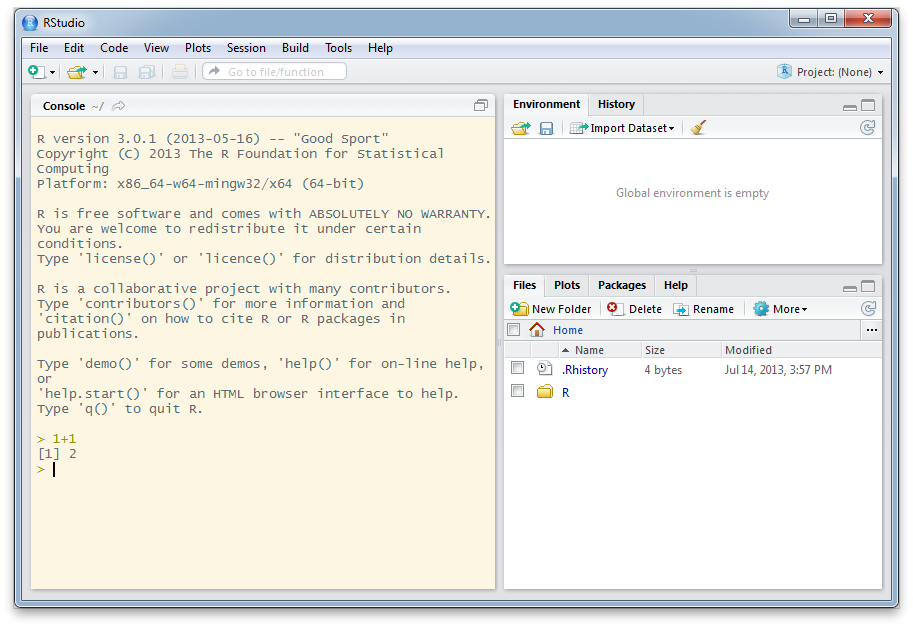
\includegraphics{figs-inc/03i-all4.png}
\caption{Here is shown the RStudio interface, after starting up and
  entering \code{1+1}.}\label{fig:rstudio}
\end{figure*}

The url for RStudio is \url{http://www.rstudio.com/}.  Click on the
icon for the downloaded installation file to install it. An RStudio
icon will appear.  Click on the icon to start RStudio.  RStudio should
find any installed version of R, and if necessary start R.  Figure
\ref{fig:rstudio} shows an RStudio display, immediately after starting
up and entering, very unimaginatively, \code{1+1}.

Technically, \marginnote{Extensive and careful RStudio documentation
  can be accessed, assuming an internet connection, from the
  \underline{Help} drop-down menu.  The notes included here are
  designed to draw attention to some of the more important RStudio
  abilities and features.}
RStudio offers an Interactive Development Environment.  It
provides, from a graphical user interface, a range of abilities that
are helpful for organizing and managing work with R.  Helpful features
of RStudio include:
\begin{itemize}
\item The organisation of work into projects.
\item The recording of files that have been accessed from RStudio, of
  help pages accessed, and of plots.  The record of files is
  maintained from one session of a project to the next.
\item By default, a miniature is displayed of any graph that is
  plotted.  A single click expands the miniature to a full graphics
  window.
\item The editing, maintenance and display of code files.
\item Abilities that assist reproducible reporting.
   \marginnote{Alternative available types of markup are R
    Markdown or R HTML or Sweave with LaTeX.}  Markup text
  surrounds R code that is incorporated into a document, with option
  settings used to control the inclusion of code and/or computer
  output in the final document. Output may include tables and graphs.
\item Abilities that help in the creation of packages.
\end{itemize}

\subsection{The RStudio file menu}

\begin{figure}
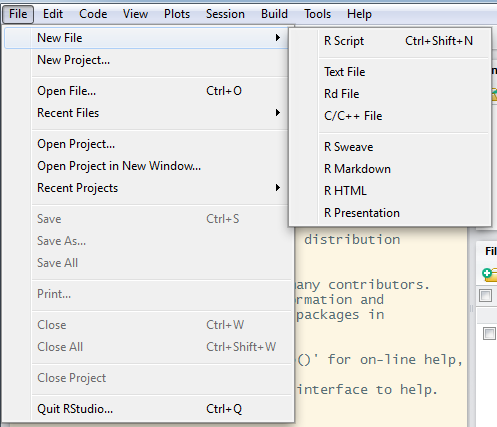
\includegraphics{figs-inc/03i-menu.png}
\caption{The RStudio \underline{File} drop-down menu.  The
  \underline{New File} submenu has been further expanded.}\label{fig:file-menu}
\end{figure}

For now, the RStudio drop-down menus that are of most immediate
importance are \underline{File} and \underline{Help}.  Here (Figure
\ref{fig:file-menu}) is the \underline{File} menu, with the
\underline{New File} submenu also shown.

Here, note the possibility of opening a new R script file, and
entering code into that file. Or, to open an existing R code file,
click on the \underline{Open File...} submenu.

The key combination <CTRL><ENTER> \marginnote{Here, <CTRL> is the
  control key and <ENTER> is the Enter key.}can be used to send code
to the command line.  Code that has been selected will be sent to the
command line.  Or if no code has been selected, the line on which the
cursor is placed will be sent to the command line.

\subsection{Compile a code notebook}

Figure \ref{fig:code-history} shows a script file in the upper left
panel.  The code has been sent to the command line, so that it also
appears in the code history panel on the upper right.

\begin{figure*}
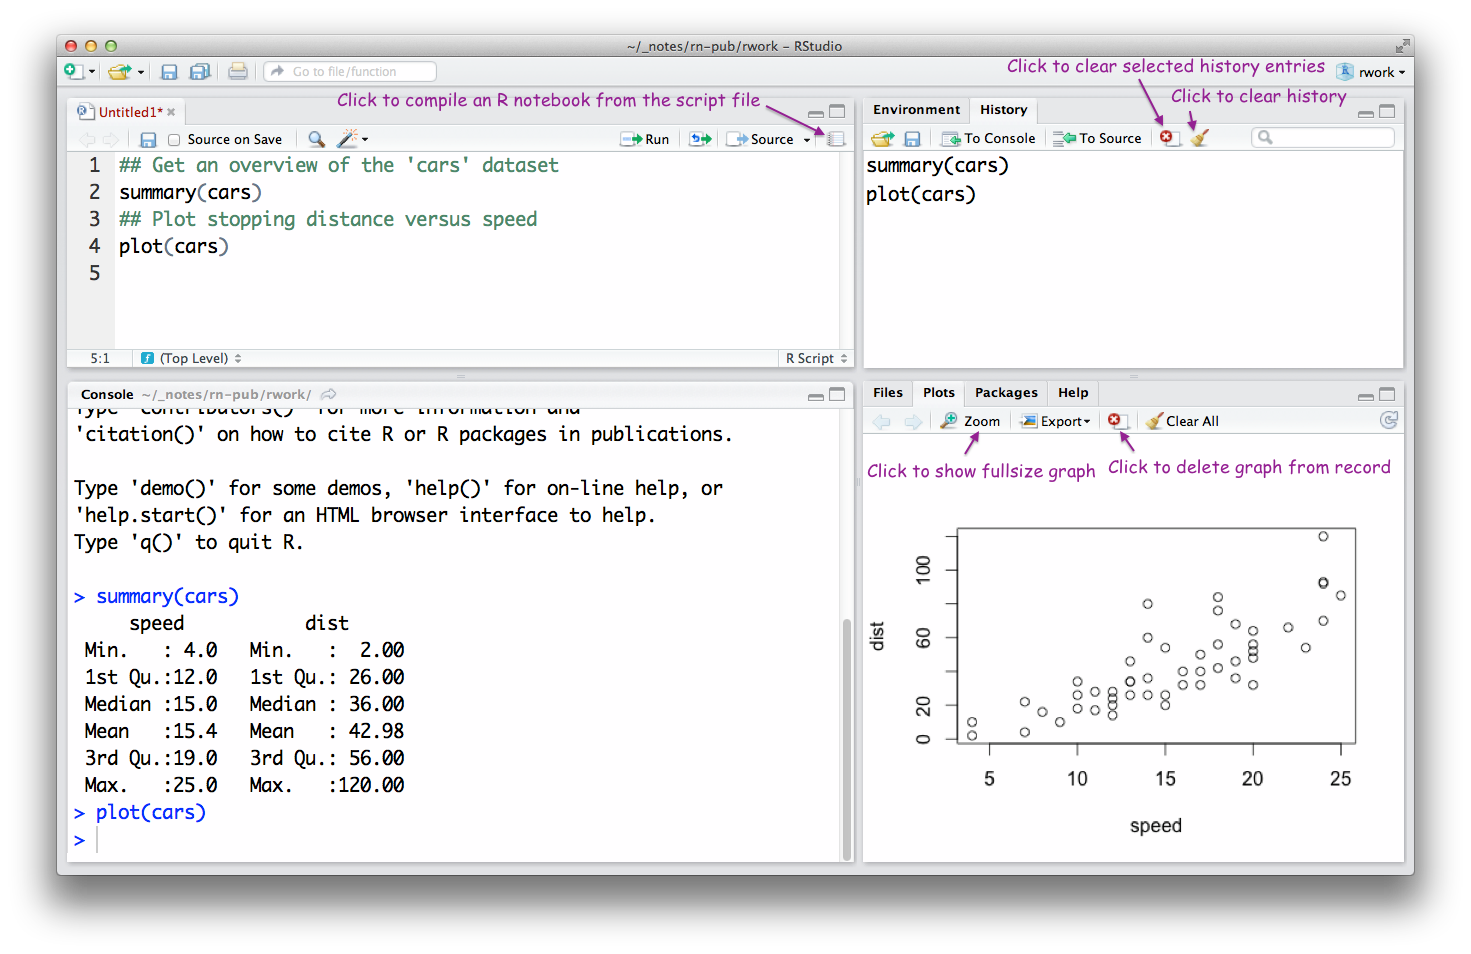
\includegraphics{figs-inc/03i-3panels.png}
\vspace*{-15pt}

\caption{Code from the script window has been sent to the command
  line.}\label{fig:code-history}
\end{figure*}

In Figure \ref{fig:code-history}, take particular note of the icon on
which you can click to create an R notebook. Upon clicking this icon,
the system will ask for a name for the file.  It will then create an
HTML file that has, along with the code and comment, the computer
output.
\marginnote{For the code that is shown, the HTML file that results
will include the output from \code{summary(cars)} and the graph from
  \code{plot(cars)}.}  An alternative to clicking on the icon is to
click on the \underline{File} drop-down menu, and then on
\underline{Compile Notebook... }.

\subsection{Managing input from the RStudio menu}\label{ss:readEtc}

Data input that is initiated from the RStudio menu uses functions
from the package \pkg{readr} for input of tabular data.
The function \code{readr::read\_table()} replaces
\code{read.table()}, \code{readr::read\_csv()} replaces
\code{read.csv()}, and similarly for other \code{read.table()}
aliases.

It uses the function \code{readxl::readxl()} for Excel
spreadsheet data. There is provision, also, using functions from
the package \pkg{haven}, to import data from SPSS (POR and
SAV files), from SAS (XPT and SAS files), and from Stata (DTA
files).  
\marginnote{See \code{vignette("semantics", package="haven")}
for details of the way that labelled data and missing values
are handled, for input from SPSS, SAS, and Stata.}

Output is in all cases to a tibble, which is a specialized form
of data frame. 
Character columns are not automatically converted to factors,
column names are not converted into valid R identifiers, and row
names are not set.  For subsequent processing, there are
important differences between tibbles and data frames that users
need to note.

\section{Abilities for reproducible reporting}
Markdown editors use simple markup conventions to control how text and
other document features will appear.  For example:
\begin{itemize}
\item[] \txtt{**Help**} or \txtt{\_\_Help\_\_} will be rendered as
\textbf{Help}
\item[] \txtt{*Help*} or \txtt{\_Help\_} will be rendered as {\em Help}.
\end{itemize}

\subsection{R Markdown}
\marginnote{R Markdown, as available under RStudio, is an enhanced
  version of Markdown.  It adds the ability to include R code,
  surrounded by markup that controls what code and/or output will appear
  in the final document.

R users are strongly encouraged to use R Markdown, or another
such markup system that allows embedded R code, for documenting any
work that is more than trivial.  Those who are familiar with
more sophisticated markdown languages may still, for some types
of work, find benefit in the simplicity and speed of working with R
markdown.}

Click on \underline{File} | \underline{New File} | \underline{R
  Markdown...}.  Clicking on HTML (alternatives are PDF, Word), on
\underline{Document} (alternatives are Presentation, Shiny, From
Template) and then on \underline{OK} displays a simple skeleton R
Markdown document thus:
\begin{verbatim}
---
title: "Untitled"
output: html_document
---

This is an R Markdown document. Markdown is a simple
formatting syntax for authoring HTML, PDF, and MS
Word documents. For more details on using R Markdown
see <http://rmarkdown.rstudio.com>.

When you click the **Knit** button a document will
be generated that includes both content as well as
the output of any embedded R code chunks within the
document. You can embed an R code chunk like this:

```{r}
summary(cars)
```

You can also embed plots, for example:

```{r, echo=FALSE}
plot(cars)
```

Note that the `echo = FALSE` parameter was added
to the code chunk to prevent printing of the R
code that generated the plot.
\end{verbatim}
\marginnote[-36pt]{For tutorial purposes, the file can
be processed as it stands.  Click the \underline{Knit HTML}
button to start the process of generating the HTML file.  When
prompted, enter a name for the file.  An HTML file will be
generated and displayed in a browser.}

In actual use, one would edit out the text and R code and replace
it with one's own text and R code chunks, then clicking on
\underline{Knit HTML}. When prompted, enter a name for the file.


\subsection*{R Markdown code chunk options}
The markup that surrounds R code can include instructions on what to
do with R code and/or any output, including tables and graphs. Should
code be executed, should it be echoed, and what output text and/or
tables and/or graphs should appear in the final document?

Here is an example of code with surrounding markup, with the
code chunk options \code{fig.width} and \code{fig.height}
giving the width and height of the initial figure, and
\code{out.width} giving the width to which it should be scaled
in the final document:
\begin{minipage}[t]{1.05\textwidth}
\begin{verbatim}
```{r plotgph, fig.width=7, fig.height=6, out.width="80%"}
plot(cars)
```
\end{verbatim}
\end{minipage}

Giving the code chunk a name, here \code{plotgph}, is optional.
\marginnote{Other possible settings include:
  \margtt{echo=FALSE} (do not show code), \&
\margtt{eval=FALSE} (do not evaluate).}
 The \code{fig.width} and \code{fig.height} settings
  control the size of the output plot, before it is scaled to fit
  within the available line width.  The \code{out.width} setting
  controls the width (here given as a percentage of the line
  width) in the final HTML document.  The width may alternatively
  be given in pixels, e.g., `out.width="600px"`.
  
An image from a file {\bf pic.png} that has been generated
separately from the markup R code can be input thus:

\begin{minipage}[t]{1.05\textwidth}
\begin{verbatim}
```{r, out.width="80%"}
knitr::include\_graphics("pic.png")
```
\end{verbatim}
\end{minipage}
  
\subsection*{$^*$Inclusion of HTML in R Markdown documents}
Note also that HTML markup can be included in R Markdown documents.
The following is a less preferred alternative to the
R code \code{knitr::include\_graphics("pic.png")} whose use was
demonstrated above:
\begin{verbatim}
<IMG SRC="pic.png" alt="Show this, if no image" STYLE="width: 1200px"/>
\end{verbatim}

The image position can if necessary be adjusted thus:
\begin{verbatim}
<IMG SRC="pic.png" alt="Show this, if no image" STYLE="position:absolute;
TOP:-25px; LEFT:40px; WIDTH:800px; HEIGHT:500px"/>
\end{verbatim}

\subsection*{R Presentation}

Note the R Presentation variant of R Markdown.
To display a simple skeleton  document, click on:
\begin{quote}
\underline{File} | \underline{New File} | \underline{R Presentation}
\end{quote}
An R Presentation document is a specific type of R Markdown document
that is formatted to provide slides that can be displayed using a
browser.

Click on \underline{Knit HTML} to process the document, either as it
stands or after replacing the sample text and code with one's own text
and code.

\subsection{$^*$Other markup types -- HTML,  LaTeX, \ldots}

\subsection*{R HTML}
\marginnote{Also available is reStructuredText (reST), which is an
  extended variant of R Markdown.}

Click on \underline{File} | \underline{New File} | \underline{R HTML}
to display a skeleton HTML document that has embedded R code.
The following shows the markup format:
\begin{verbatim}
<!--begin.rcode fig.width=7, fig.height=6, out.width="600px"
plot(cars)
end.rcode-->
\end{verbatim}

Again, the document that appears can be processed as it stands --
click on \underline{Knit HTML}.

\subsection*{R Sweave: }

Click on \underline{File} | \underline{New
  File} | \underline{R Sweave} to display a template for a LaTeX file.
The web page \url{http://maths-people.anu.edu.au/~johnm/r-book/knitr/} has
files that demonstrate the use of {\em knitr} Sweave type markup.

\subsection{RStudio documentation -- markup and other}

Extensive RStudio documentation is available online.  Click on
\underline{Help} | \underline{RStudio Docs} to go to the relevant web
page. For \underline{R Markdown} and \underline{R Presentation}, note
the documentation files for {\bf Using R Markdown}.  \LaTeX\ users
should note the {\bf Sweave and knitr} documentation files.

\subsection{A strategy for RStudio project management}

RStudio is designed to encourage good project management practices,
using a strategy akin to the following:
\begin{itemize}
\item[] Set up each new project in its own working directory.
\item[] For each project, maintain one or more script files that
holds the code.  Script files can be compiled into "notebooks"
for purposes of keeping a paper record.
\item[] Script files are readily expanded into R Markdown documents
-- a simple form of "reproducible reporting" document.  They can
as required be expanded into a draft for a paper.
\end{itemize}


\section{Summary and Exercises}

\subsection{Summary}
\begin{itemizz}
\item[] Each R session has a working directory, where R will by
  default look for files or store files that are external to R.
\item[]
\marginnote{From within functions, R will look first in the
functions environment, and then if necessary look within the
search list.}
User-created R objects are added to the workspace, which is
at the base of a search list, i.e., a list of `databases' that R
will search when it looks for objects.
\item[] It is good practice to keep a separate workspace and
  associated working directory for each major project.  Use script
  files to keep a record of work.  \marginnote{Before making big
    changes to the workspace, it may be wise to save the
    existing workspace under a name (e.g., \margtt{Aug27.RData})
    different from the default \margtt{.RData}.}
\item[] At the end of a session an image of the workspace will
  typically (respond `\code{y}' when asked) be saved into the working
  directory.
\item[] Note also the use of \code{attach()} to give access to objects
  in an image (\textbf{.RData} or \textbf{.rda})
  file.\sidenote{Include the name of the file (optionally preceded by
    a path) in quotes.}
\item[] R has an extensive help system.  Use it!
\end{itemizz}

\subsection{Exercises}\label{ss:wd}
\marginnote{The function \margtt{DAAG::datafile()} is able to
place in the working directory any of the files: {\bf fuel.txt}
{\bf molclock1.txt}, {\bf molclock2.txt},  {\bf travelbooks.txt}.
Specify, e.g.\\
\margtt{datafile(file="fuel")}}
Data files used in these exercises are available from the web
page  \url{http://www.maths-people.anu.edu.au/~johnm/datasets/text/}.

\begin{enumerate}
\item
Place the file \textbf{fuel.txt} to your working directory.
\item Use \code{file.show()} to examine the file, or click on the
  RStudio \underline{Files} menu and then on the file name to display
  it.  Check carefully whether there is a header line.  Use the
  RStudio menu to input the data into R, with the name \code{fuel}.
  Then, as an alternative, use \code{read.table()} directly.  (If
  necessary use the code generated by RStudio as a crib.)  In each
  case, display the data frame and check that data have been input
  correctly.
\item \marginnote{A shortcut for placing these files in the working
    directory is:\\
    \margtt{datafile(file=c("molclock1",}\\
    \hfill \margtt{"molclock2"))}} Place the files
  \textbf{molclock1.txt} and \textbf{molclock2.txt} in a directory
  from which you can read them into R.  As in Exercise 1, use the
  RStudio menu to input each of these, then using
  \code{read.table()} directly to achieve the same result.  Check,
  in each case, that data have been input correctly.

  Use the function \code{save()} to save \code{molclock1}, into an R
  image file.  Delete the data frame \code{molclock1}, and check that
  you can recover the data by loading the image file.\label{ex:mol1}
\item The following counts, for each species, the number of missing values
for the column \code{root} of the data frame \code{DAAG::rainforest}:
\begin{knitrout}
\definecolor{shadecolor}{rgb}{0.969, 0.969, 0.969}\color{fgcolor}\begin{kframe}
\begin{alltt}
\hlkwd{library}\hlstd{(DAAG)}
\hlkwd{with}\hlstd{(rainforest,} \hlkwd{table}\hlstd{(}\hlkwd{complete.cases}\hlstd{(root), species))}
\end{alltt}
\end{kframe}
\end{knitrout}
For each species, how many rows are ``complete'', i.e., have no values
that are missing?
\item For each column of the data frame \code{MASS::Pima.tr2},
determine the number of missing values.
\item The function \code{dim()} returns the dimensions (a vector that
 has the number of rows, then number of columns) of data frames and
 matrices.  Use this function to find the number of rows in the data
 frames \code{tinting}, \code{possum} and \code{possumsites}
 (all in the \pkg{DAAG} package).
\item Use \code{mean()} and \code{range()} to find the
mean and range of:
\begin{itemize}
  \item[(a)] the numbers 1, 2, \ldots, 21
  \item[(b)] the sample of 50 random normal values, that can be generated
    from a normaL distribution with mean 0 and variance 1 using the
    assignment \code{y <- rnorm(50)}.
  \item[(c)]
\marginnote{The \pkg{datasets} package
    that has the data frame \margtt{women} is by default attached when R is
    started.}
the columns \code{height} and \code{weight} in the
    data frame \code{women}.
\end{itemize}
Repeat (b) several times, on each occasion generating a nwe set of
50 random numbers.
\item Repeat exercise 6, now applying the functions \code{median()} and
\code{sum()}.
\item Extract the following subsets from the data frame \code{DAAG::ais}
\begin{itemize}
\item[(a)] Extract the data for the rowers.
\item[(b)] Extract the data for the rowers, the netballers and the
tennis players.
\item[(c)] Extract the data for the female basketballers and rowers.
\end{itemize}
\item Use \code{head()} to check the names of the columns, and the first
few rows of data, in the data frame \code{DAAG::rainforest}.
Use \verb!table(rainforest$species)! to check the names and numbers of
each species that are present in the data.
The following extracts the rows for the species `Acmena smithii'
\begin{knitrout}
\definecolor{shadecolor}{rgb}{0.969, 0.969, 0.969}\color{fgcolor}\begin{kframe}
\begin{alltt}
\hlstd{Acmena} \hlkwb{<-} \hlkwd{subset}\hlstd{(rainforest, species}\hlopt{==}\hlstr{"Acmena smithii"}\hlstd{)}
\end{alltt}
\end{kframe}
\end{knitrout}
The following extracts the rows for the species `Acacia mabellae' and
`Acmena smithii':
\begin{fullwidth}

\begin{knitrout}
\definecolor{shadecolor}{rgb}{0.969, 0.969, 0.969}\color{fgcolor}\begin{kframe}
\begin{alltt}
\hlstd{AcSpecies} \hlkwb{<-} \hlkwd{subset}\hlstd{(rainforest, species} \hlopt \hlkwd{c}\hlstd{(}\hlstr{"Acacia mabellae"}\hlstd{,}
                                               \hlstr{"Acmena smithii"}\hlstd{))}
\end{alltt}
\end{kframe}
\end{knitrout}

\end{fullwidth}
Now extract the rows for all species except `C. fraseri'.
\end{enumerate}
\cleartooddpage
